%************************************************
\chapter{The Planner and Plan Knowledge}
\label{chapter:the_planner_and_plan_knowledge}
%************************************************



\section{Plan Operators}

Plans are composed of four basic types of plan operators.
\begin{enumerate}
\item The \emph{resource activation operator} references a
  counterfactual transframe, which includes specific resource
  activation dependencies as well as specific hypothesis dependencies.
\item The \emph{resource suppression operator} references a resource
  that should be suppressed when this operator is executed.
\item The \emph{sequential program operator} temporally orders two
  other plan operators.
\item The \emph{parallel program operator} arranges two other plan
  operators to be executed simultaneously.
\end{enumerate}
{\mbox{\autoref{figure:example_plan_operators}}} shows an example of a
plan with four composable plan operators, while
{\mbox{\autoref{figure:example_plan}}} shows a more detailed example
of a two-step plan.
\begin{figure}
\centering
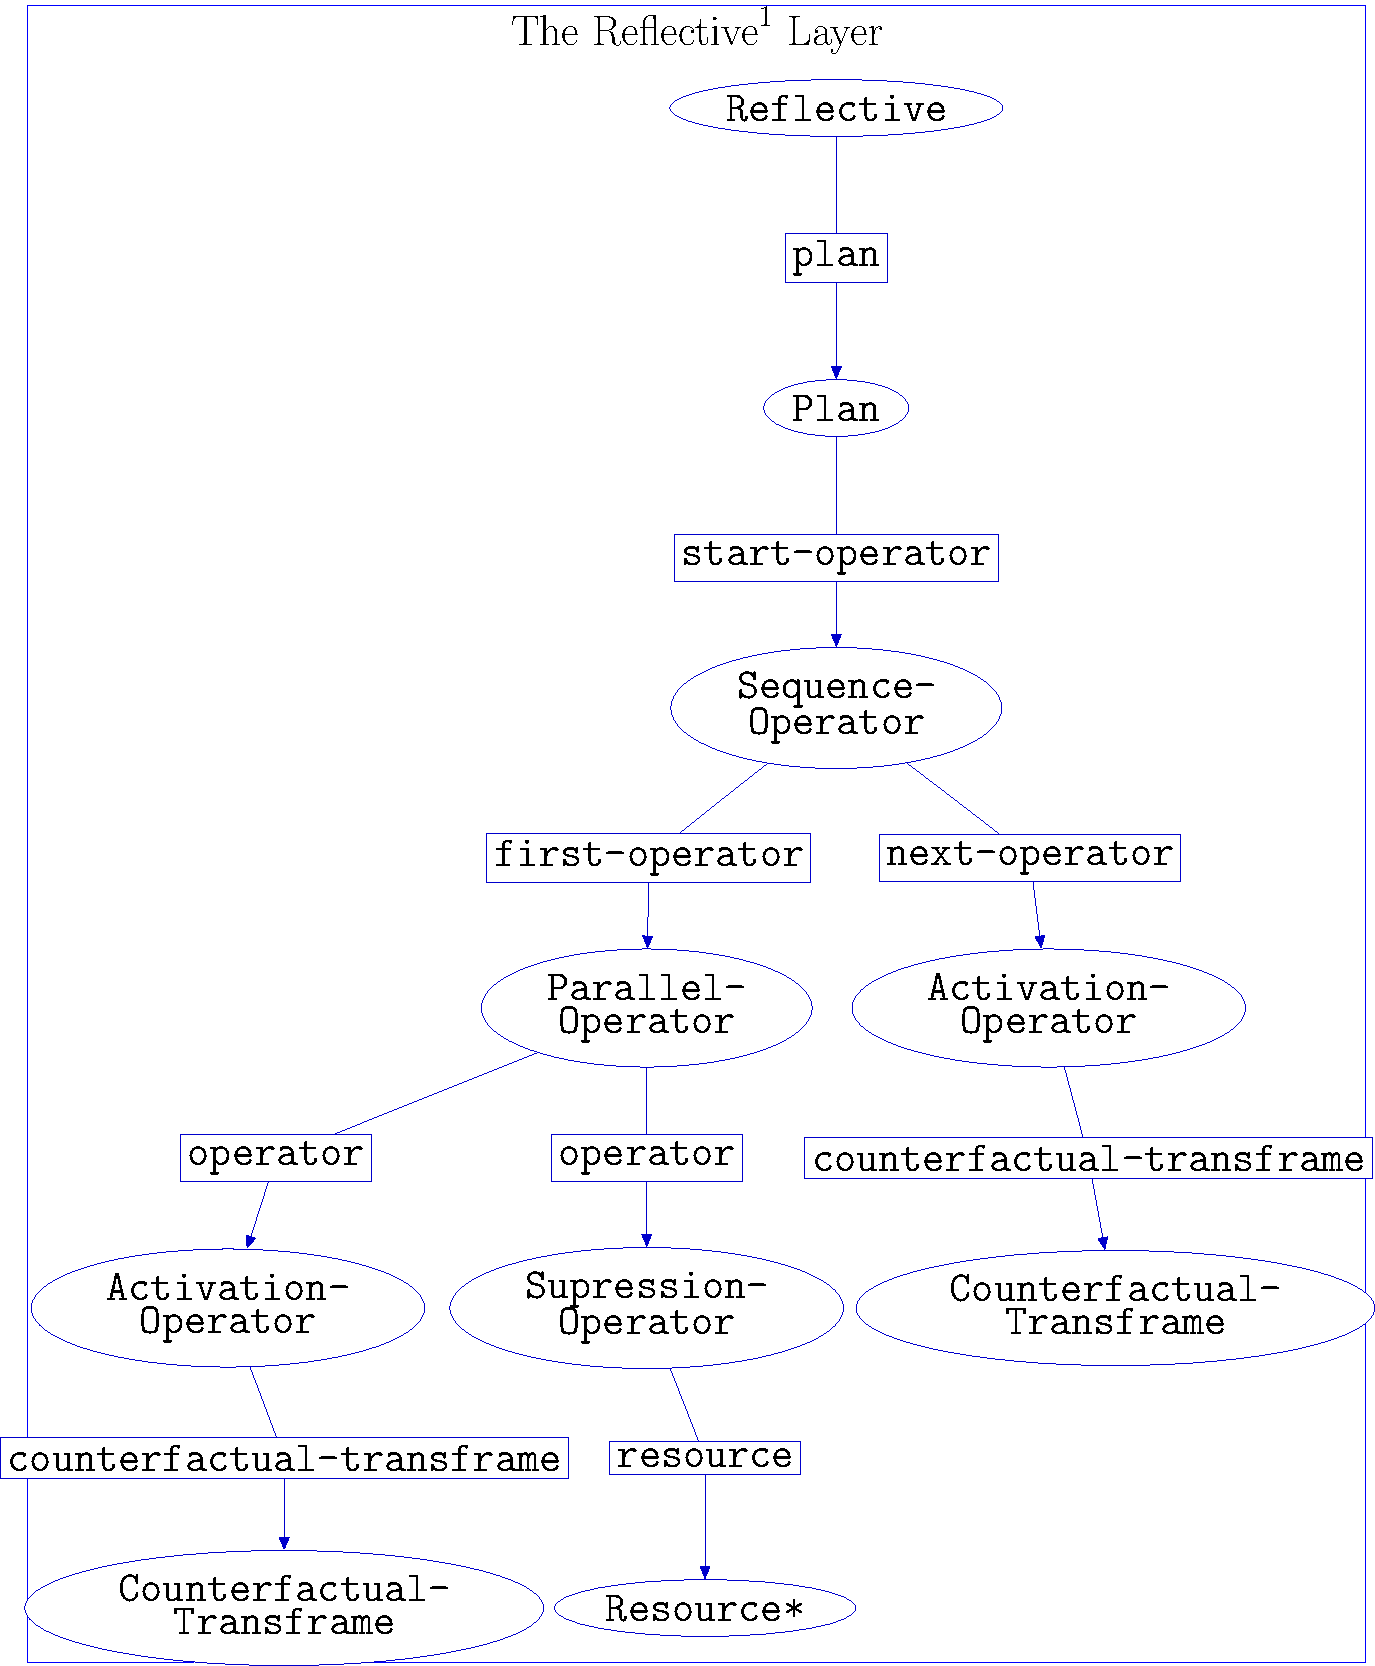
\includegraphics[width=12cm]{gfx/example_plan_operators}
\caption[An example of a plan with four composable plan operators.]{An
  example of a plan with four basic plan operators: (1) the resource
  activation operator, (2) the resource suppression operator, (3) the
  sequential program operator, and (4) the parallel program operator.}
\label{figure:example_plan_operators}
\end{figure}
\begin{figure}
\hspace*{-4cm}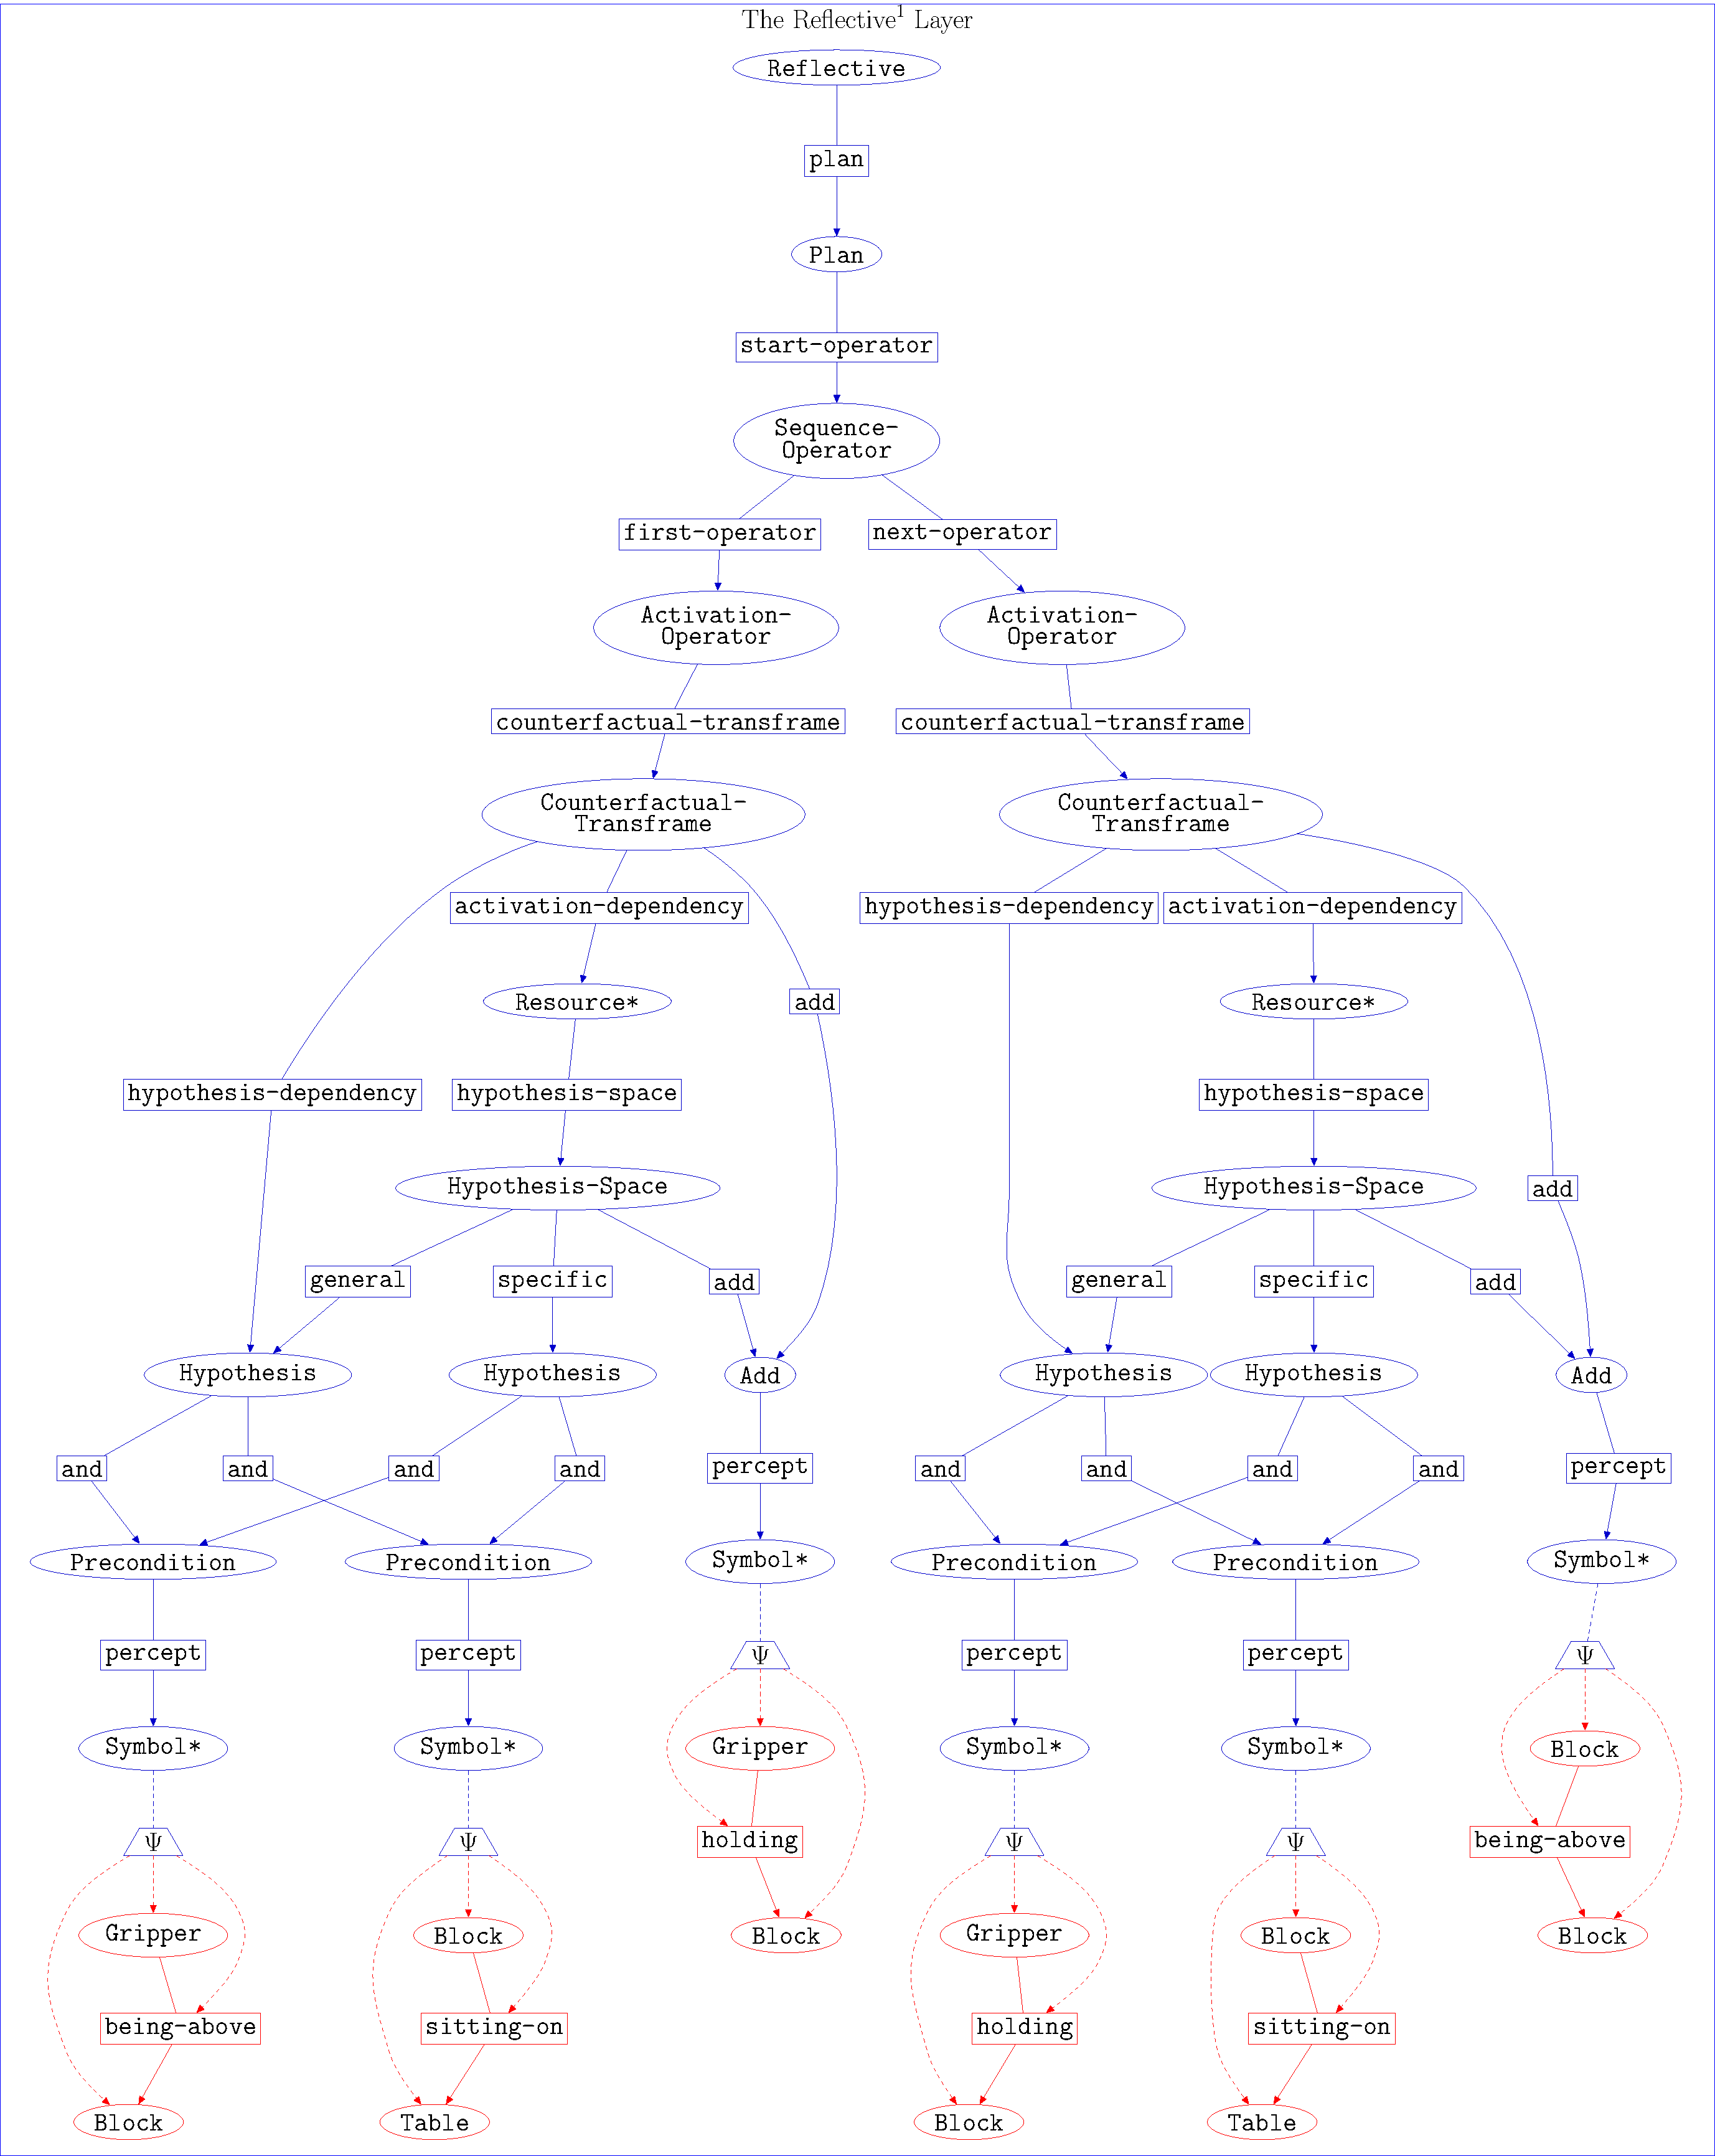
\includegraphics[width=18cm]{gfx/example_plan}
\caption[An example of a two-step plan.]{An example of a two-step
  plan.}
\label{figure:example_plan}
\end{figure}

\section{A Planner}

The first-order reflective thinking layer makes plans in order to make
plans that will accomplish symbolic physical goals when executed.
{\mbox{\autoref{figure:example_planner}}} shows an example of a
planner.  In the model, a planner is a simple computational machine
with different registers that creates and manipulates plan objects.
The operations of a first-order planner can be seen as symbolic
resources in the second-order reflective thinking layer.  In general,
planning operations can be any kind of dynamic activity of the
first-order reflective thinking layer.  Because the model is not yet
advanced enough to abstract objects and their subjective perspectives,
this planning machine the resources in the second-order reflective
layer resemble the simple symbolic actions of a RISC processor, which
are like the symbolic bytecodes of a virtual machine.  The simplest
symbolic resources in the second-order reflective layer are the
following list of actions that simply move plans between the different
registers of the planning machine:
\begin{itemize}
\item {\tt focus-on-register-a*}: Copy the plan in {\tt register-a} to
  the {\tt focus} register.
\item {\tt focus-on-register-b*}: Copy the plan in {\tt register-b} to
  the {\tt focus} register.
\item {\tt focus-on-execution*}: Copy the plan in the {\tt execute}
  register to the {\tt focus} register.
\item {\tt copy-focus-to-register-a*}: Copy the plan in the {\tt
  focus} register to register {\tt a}.
\item {\tt copy-focus-to-register-b*}: Copy the plan in the {\tt
  focus} register to register {\tt b}.
\item {\tt execute-plan-in-focus*}: Copy the plan in the {\tt focus}
  register to the {\tt execute} register.
\item {\tt execute-plan-in-focus*}: Copy the plan in the {\tt focus}
  register to the {\tt execute} register.
\item {\tt stop-execution*}: Remove any plan from the {\tt execute}
  register.
\end{itemize}
\begin{figure}
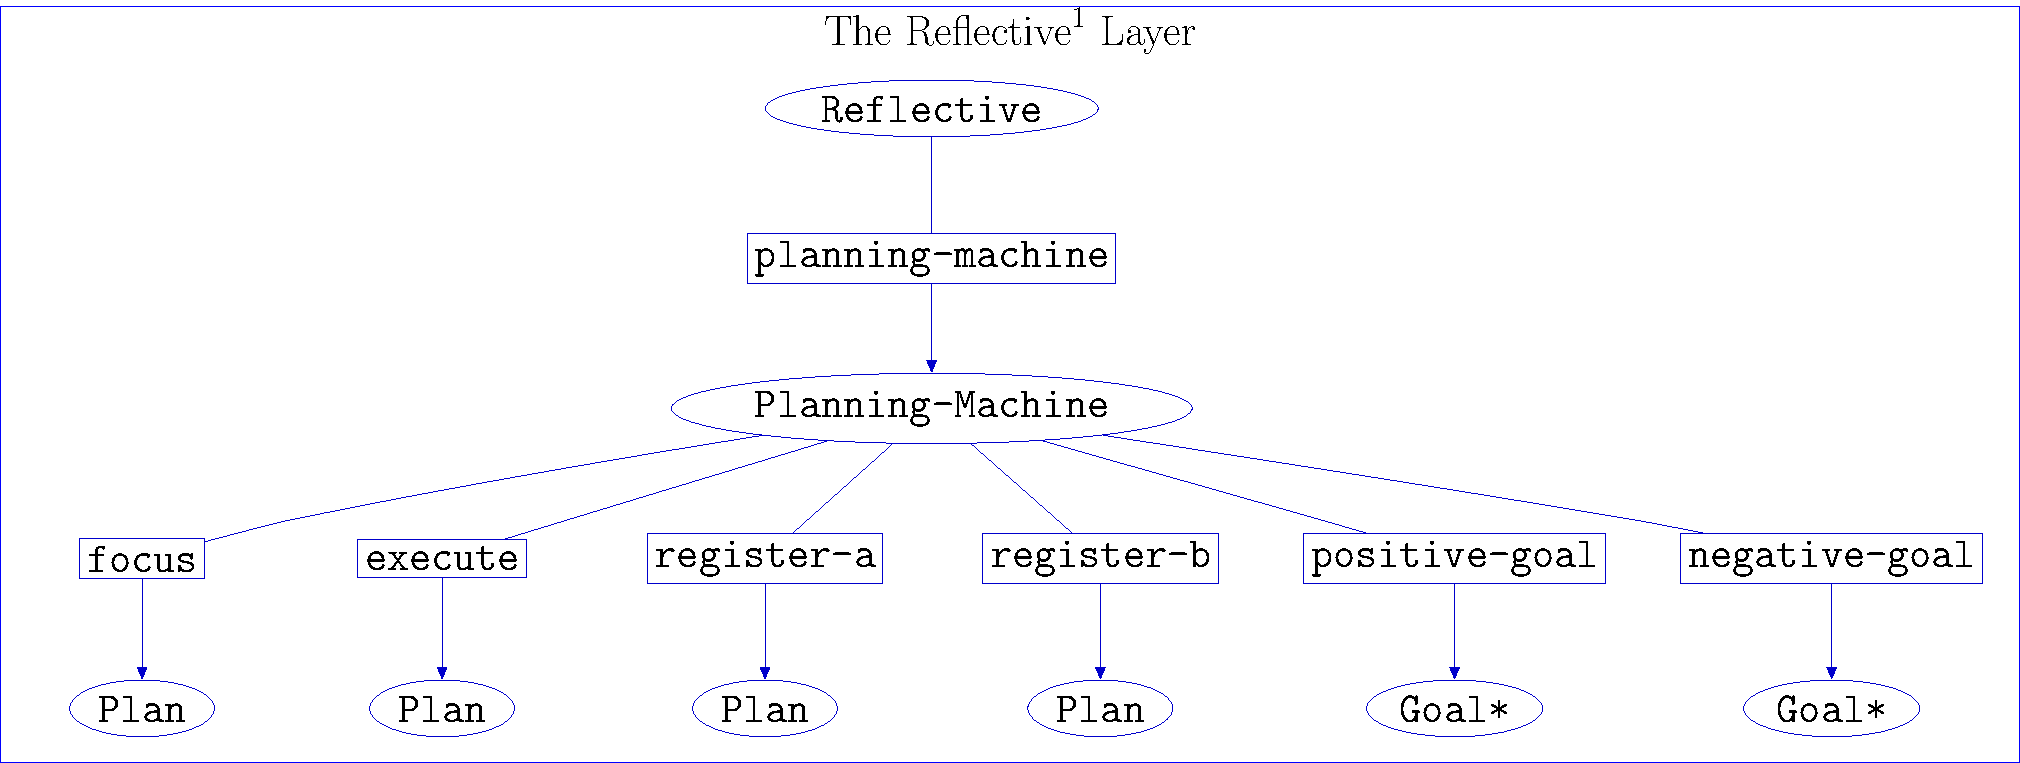
\includegraphics[width=12cm]{gfx/example_planner}
\caption[An example of a planner.]{An example of a planner.}
\label{figure:example_planner}
\end{figure}
The planner's execution register is a special register that holds the
plan that is currently executing.  As the planner is like a virtual
machine, plans are like computer programs for this virtual machine.
The planner has a number of activities that create plans that
accomplish or avoid the current goals in the {\tt positive-goal} and
{\tt negative-goal} slots of the planner.  These activities are seen
as symbolic resources that can be used to accomplish planning goals by
the second-order reflective thinking layer.  Some of these plan
creation and manipulation resources in the second-order reflective
thinking layer are as follows:
\begin{itemize}
\item {\tt create-empty-plan*}: Create new plan with no operators and
  place in the {\tt focus} register.
\item {\tt extend-plan-greedy*}: Create new plan in the {\tt focus}
  register by adding a resource activation operator to the end of a
  duplicate of the plan in {\tt register-a}.  The new activation
  operator is chosen using a greedy technique that compares the
  options with a heuristic.
\item {\tt sequence-plans*}: Create new plan in the {\tt focus}
  register with a sequential program operator that orders a duplicate
  of the plan in {\tt register-a} as the {\tt first-operator} and a
  duplicate of the plan in {\tt register-b} as the {\tt
    next-operator}.
\item {\tt parallelize-plans*}: Create new plan in the {\tt focus}
  register with a parallel program operator that contains duplicates
  of the plans in {\tt register-a} and {\tt register-b}.
\item {\tt reverse-sequence*}: Create new plan in the {\tt focus}
  register with the reverse of a sequence operator in the plan in {\tt
    register-a}.  \cite{sussman:1973} mentions a related planning bug
  where preconditions of one action clobbers the preconditions of
  another, where the solution is sometimes simply reversing the
  actions in the plan.
\item {\tt parallelize-sequence*}: Create new plan in the {\tt focus}
  register replacing a parallel program operator with a sequence
  operator in the plan in {\tt register-a}.
\end{itemize}
These first-order reflective planning operators can be used by the
second-order reflective layer in order to make second-order plans that
control the first-order planner.

\section{Symbolizing Goals}

Positive and negative first-order planner goals are symbolized from
the $\text{reflective}^0$ layer of physical activity.  Note the
bottom-up type of goal-oriented control in the model.  Also, because
reflective thinking layers are thought of as running concurrently in
the model, there is no necessary priority for devoting thinking
resources to any specific layer of thinking as more important than
another.  The implementation includes built-in goals that have already
been symbolized as positive goals that are included as part of the
first-order reflective planner.

\section{Second-order Resources}

The second-order reflective layer is the lowest layer that is able to
symbolize references to the dynamic activities of reflective thinking.
Although not included in the implementation, here is a list of
examples of symbolic resources that could exist in the reflective
thinking layers of order two or greater:
\begin{itemize}
\item {\tt refine-symbolic-perception*}: Create a new symbol that
  divides the currently perceived symbols into smaller subgraphs of
  dynamic activity that may be helpful for accomplishing or avoiding
  the positive and negative goals currently in the planner.
\item {\tt refine-symbolic-resource*}: Create a new symbol that refers
  to a subgraph of the current symbolic resource references.
\item {\tt create-type-perception*}: Create a new symbol that refers
  to the logical ``or'' or disjoint perception of two or more symbolic
  perceptual references.
\item {\tt create-analogical-plan*}: Create a new plan in the {\tt
  focus} register that satisfies the \cite{winston:1970}
  difference-of-differences relationship between the plans in {\tt
    register-a} and {\tt register-b} when applied to {\tt register-c}.
  This algorithm has been implemented by Panupong Pasupat and is
  included in the ``analogy'' package of the implementation, but is
  not included in my proof of concept demonstrative example.
\end{itemize}
\cite{singh:2003, singh:2005a} describe a variety of first-order and
second-order reflective resources, many of which assume an object
oriented social model, but some of which could help to augment the
more basic $n$ layers of reflective thinking in this model.


%\section{Counterfactual Simultaneities}
%
%Learned hypothetical transframes allow the creation of hypothetical
%future simultaneities that depend on two things: (1) action resources
%to be activated, and (2) sets of resource specific general and
%resource specific transframe hypotheses continuing to be consistent
%with factual knowledge.
%{\mbox{\autoref{figure:example_counterfactual_simultaneity}}} shows an
%example of a counterfactual simultaneity.
%\begin{figure}
%\center
%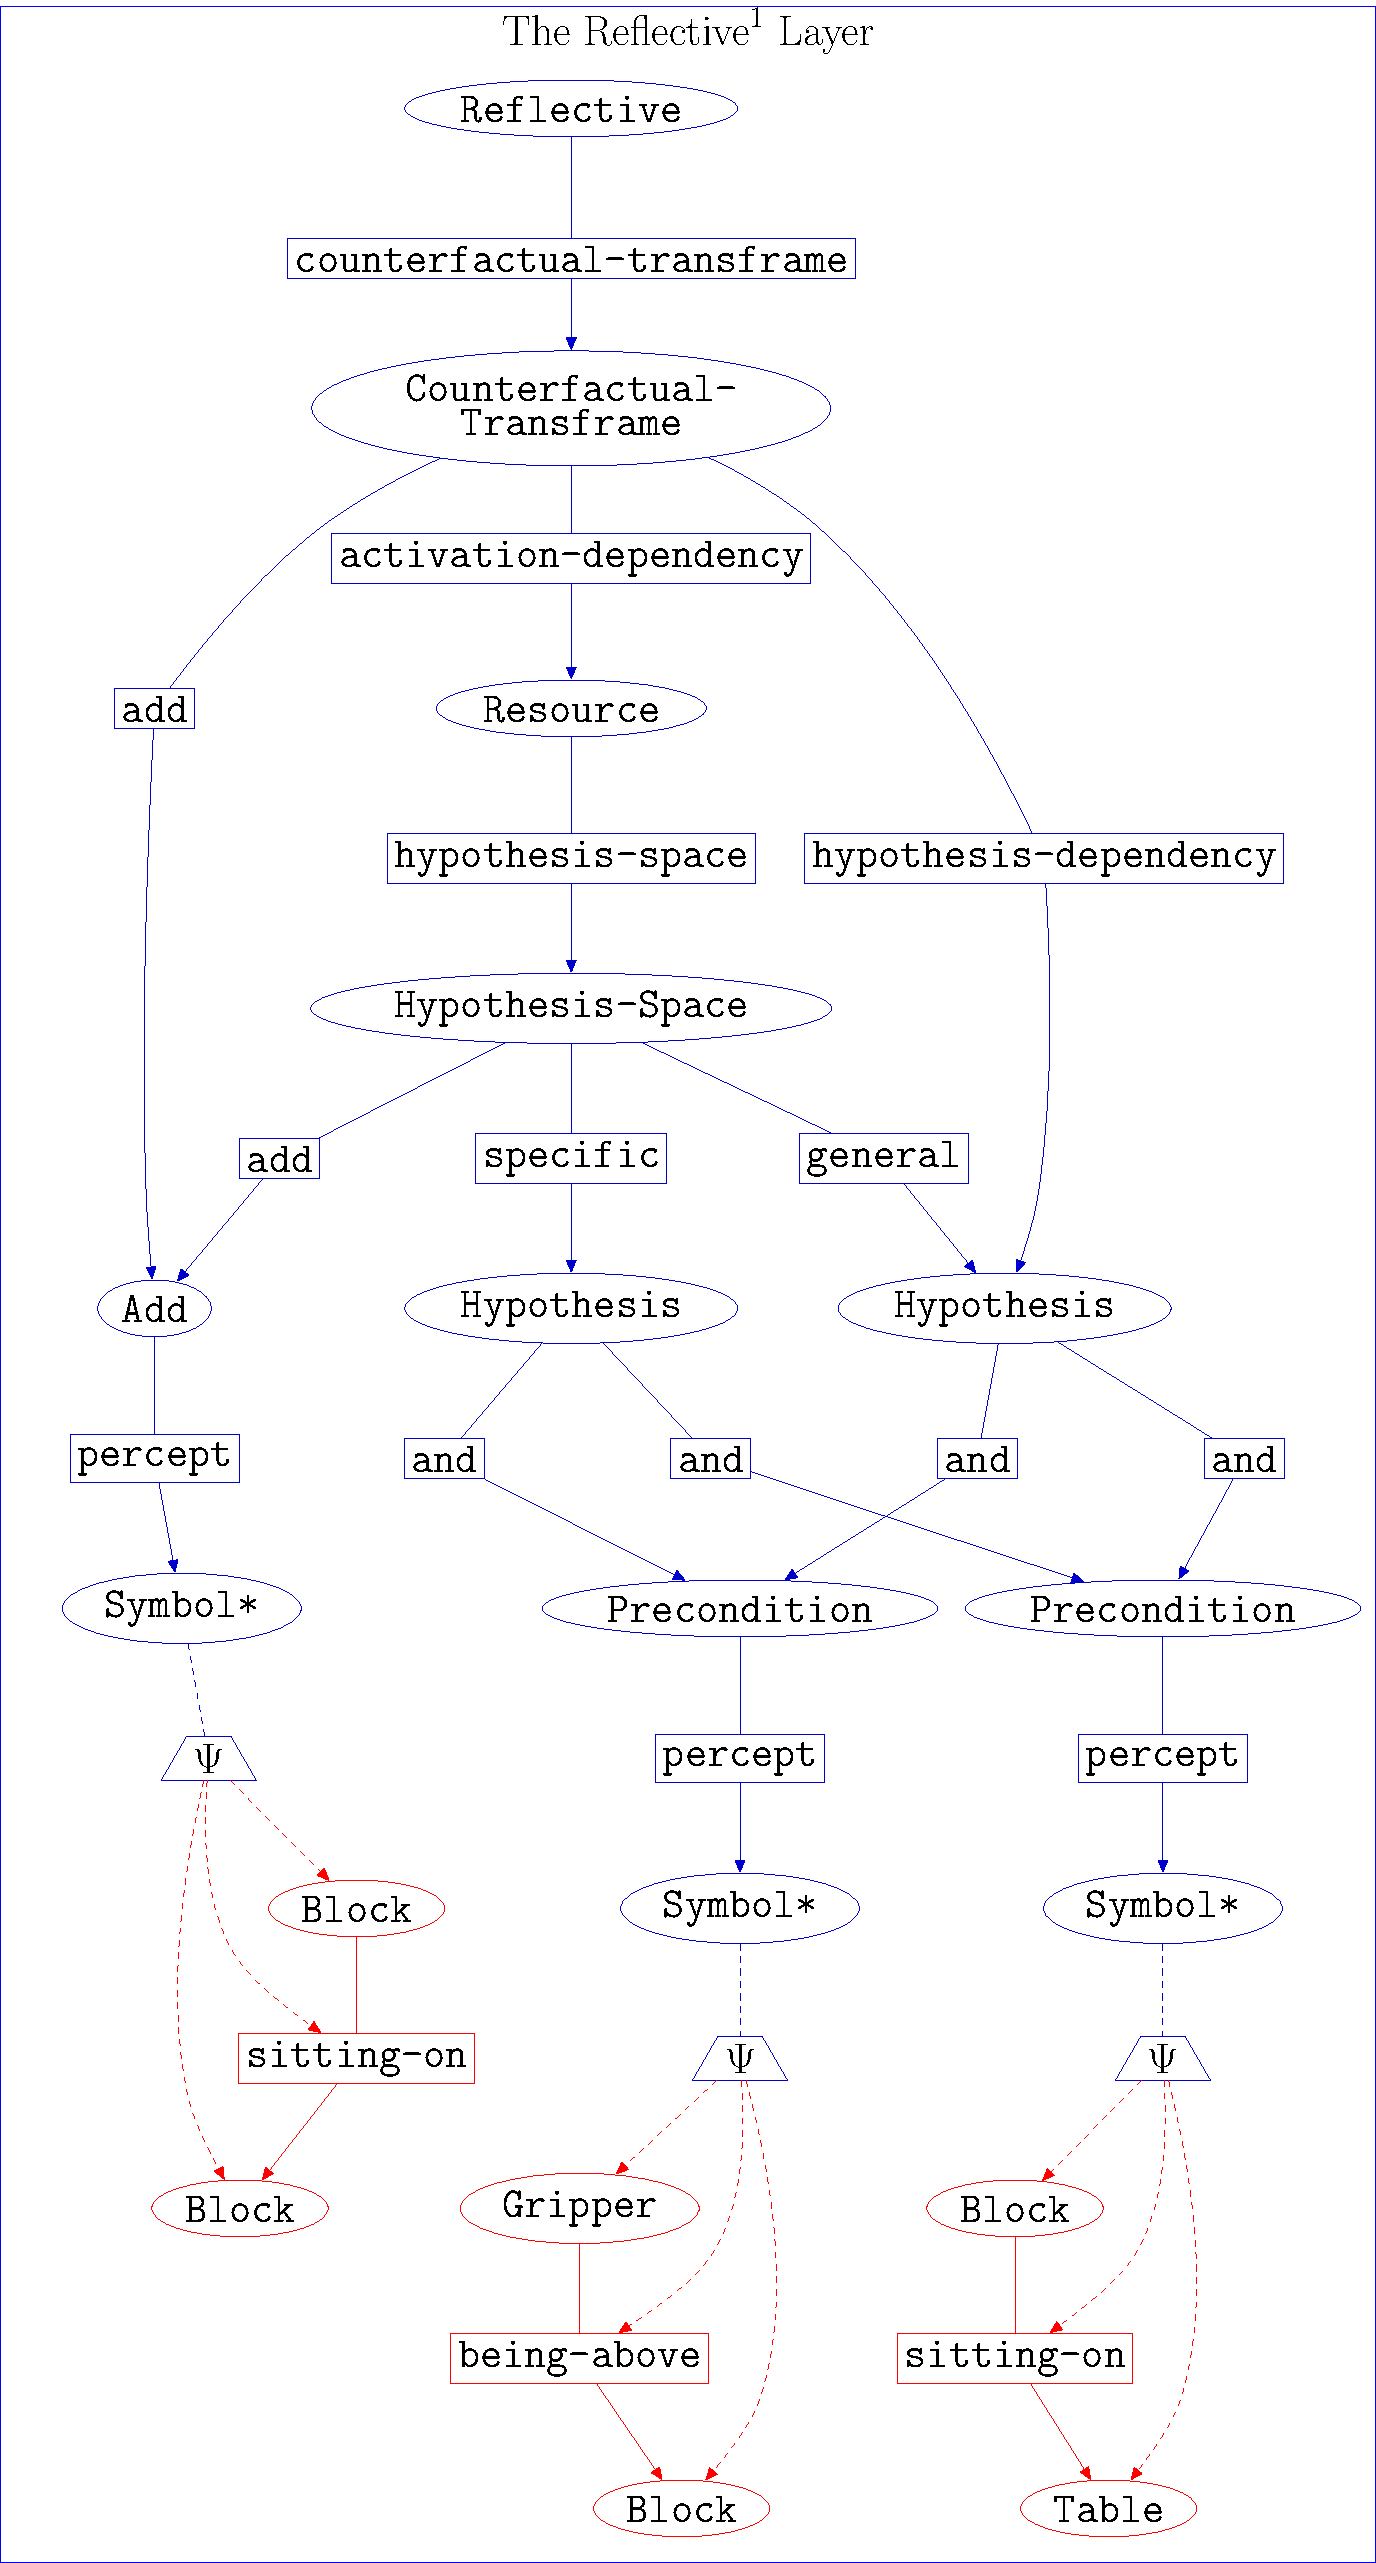
\includegraphics[width=12cm]{gfx/example_counterfactual_simultaneity}
%\caption[An example of a counterfactual simultaneity.]{An example of a
%  counterfactual simultaneity.}
%\label{figure:example_counterfactual_simultaneity}
%\end{figure}


%\section{Causal Knowledge}

%Now that a separate temporal sequence for each reflective layer has
%been defined, this factual grounded knowledge can be abstracted into
%hypothetical causal models that are useful for planning toward goals
%in a counterfactual future.



%{\mbox{\autoref{figure:example_causal_knowledge}}} shows an example of
%causal knowledge.
%\begin{figure}
%\center
%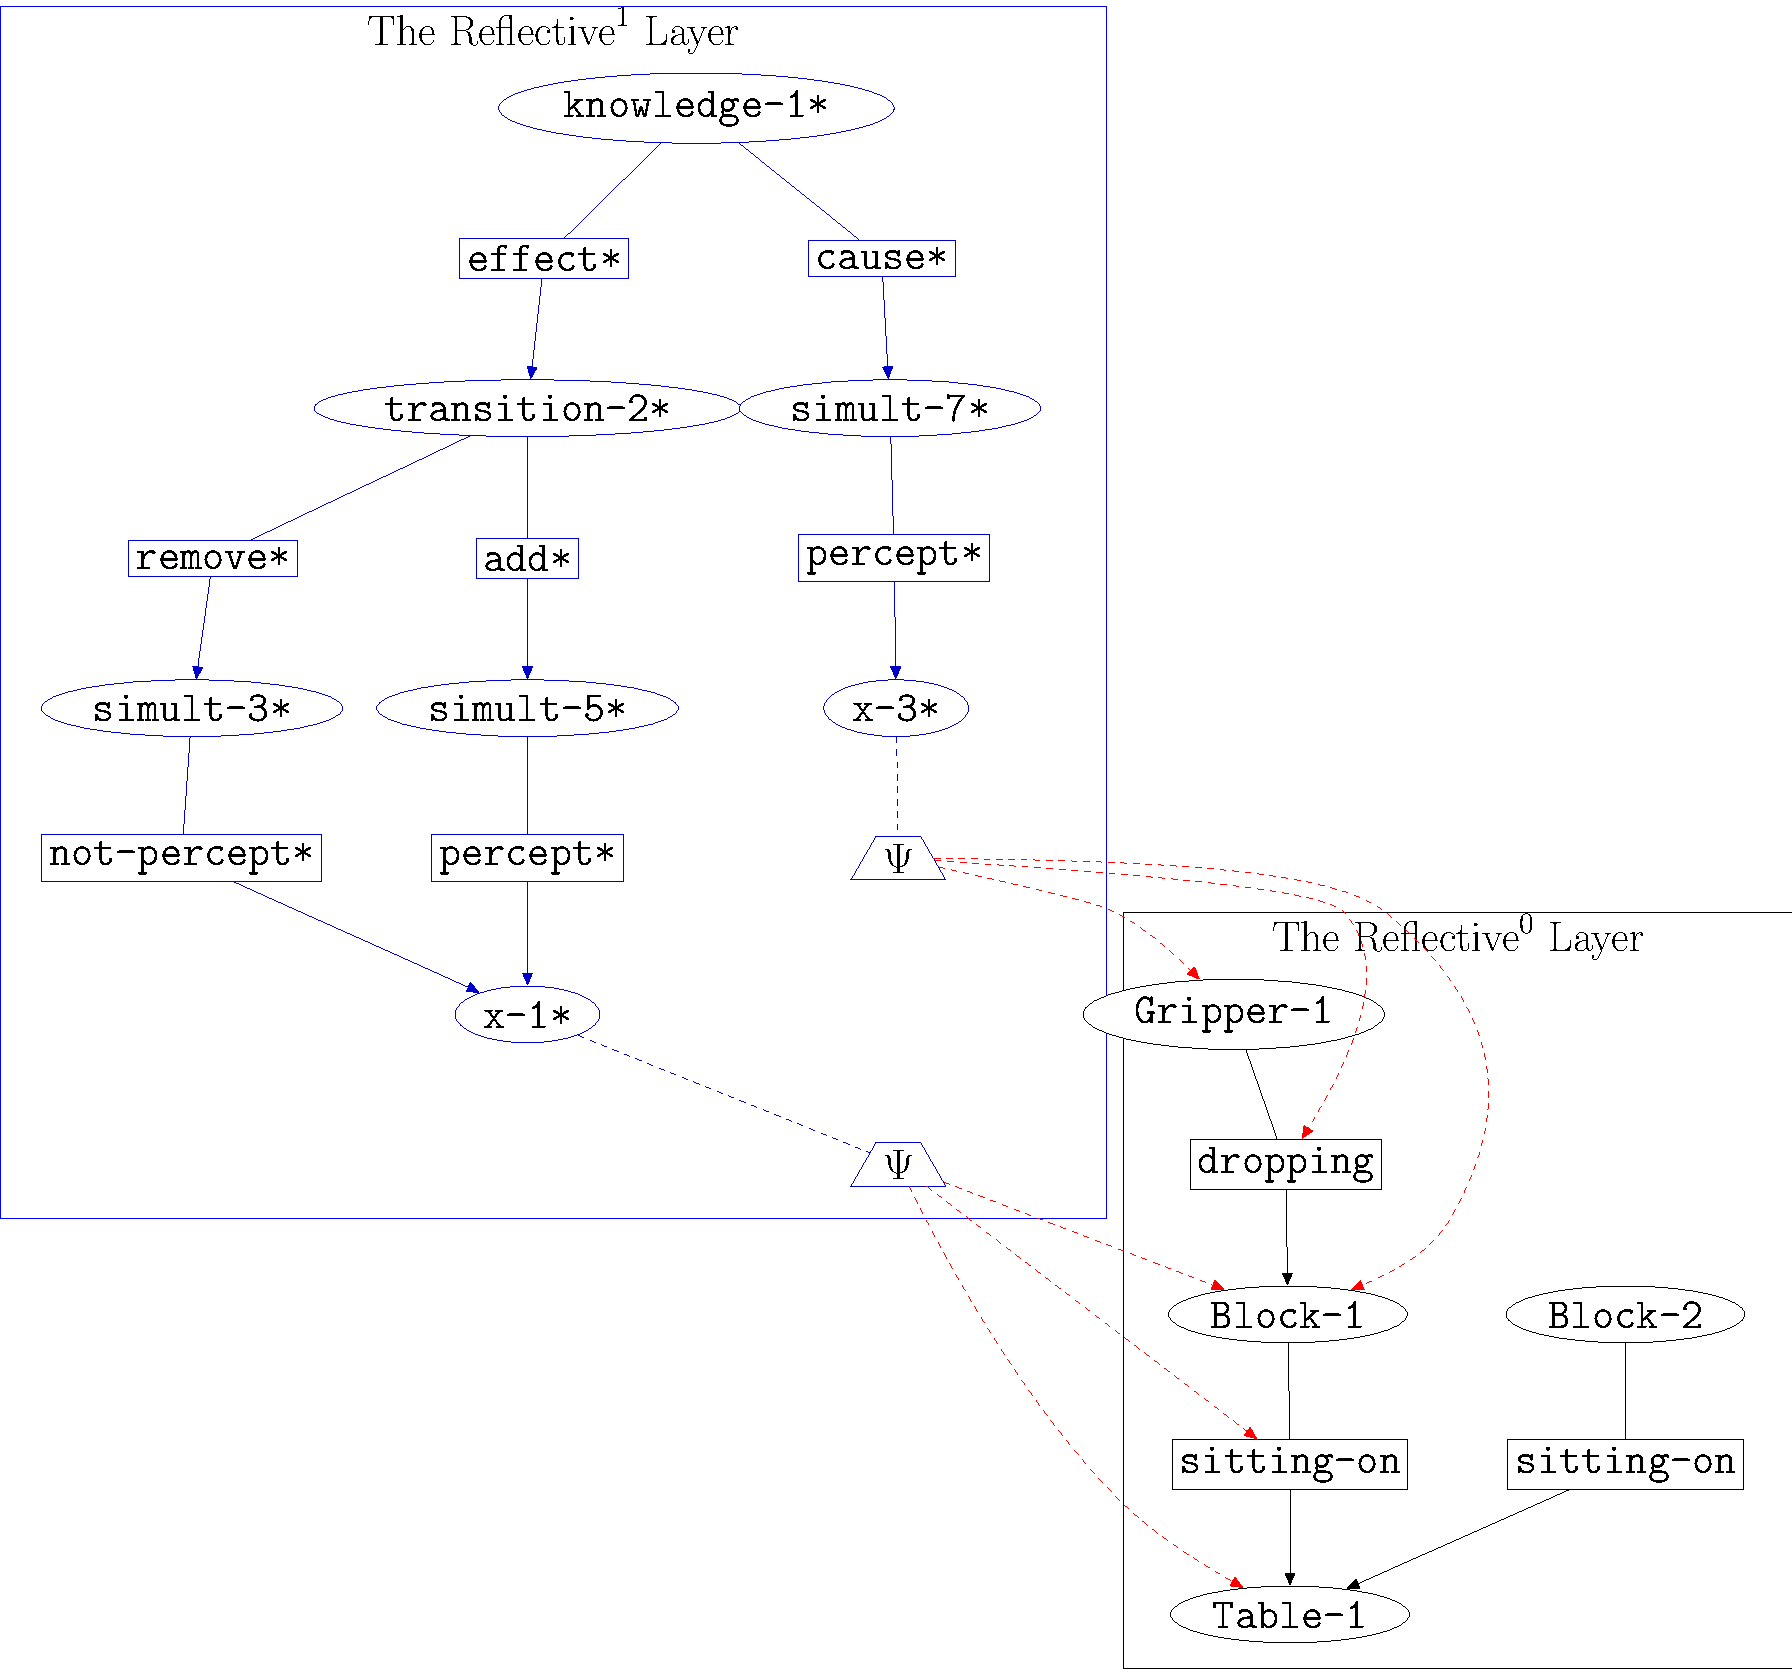
\includegraphics[width=12cm]{gfx/example_causal_knowledge}
%\caption[An example of a causal knowledge.]{An example of causal
%  knowledge, $\text{\tt{knowledge}}_1^*$, where the simultaneity,
%  $\text{\tt{simult}}_7^*$, is known to be the cause of the
%  transframe, $\text{\tt{transition}}_2^*$.  Negative perceptions are
%  omitted here for to reduce visual clutter.}
%\label{figure:example_causal_knowledge}
%\end{figure}

%\section{Representing Causal Hypotheses}

%{\mbox{\autoref{figure:example_causal_hypothesis}}} shows an example
%of a causal hypothesis, $h_1^*$, where the simultaneity,
%$\text{\tt{simult}}_7^*$, is hypothesized to be the cause of the
%transframe, $\text{\tt{transframe}}_2^*$.  In other words, the gripper
%dropping the block causes the block to be sitting on the table.
%\begin{figure}
%\center
%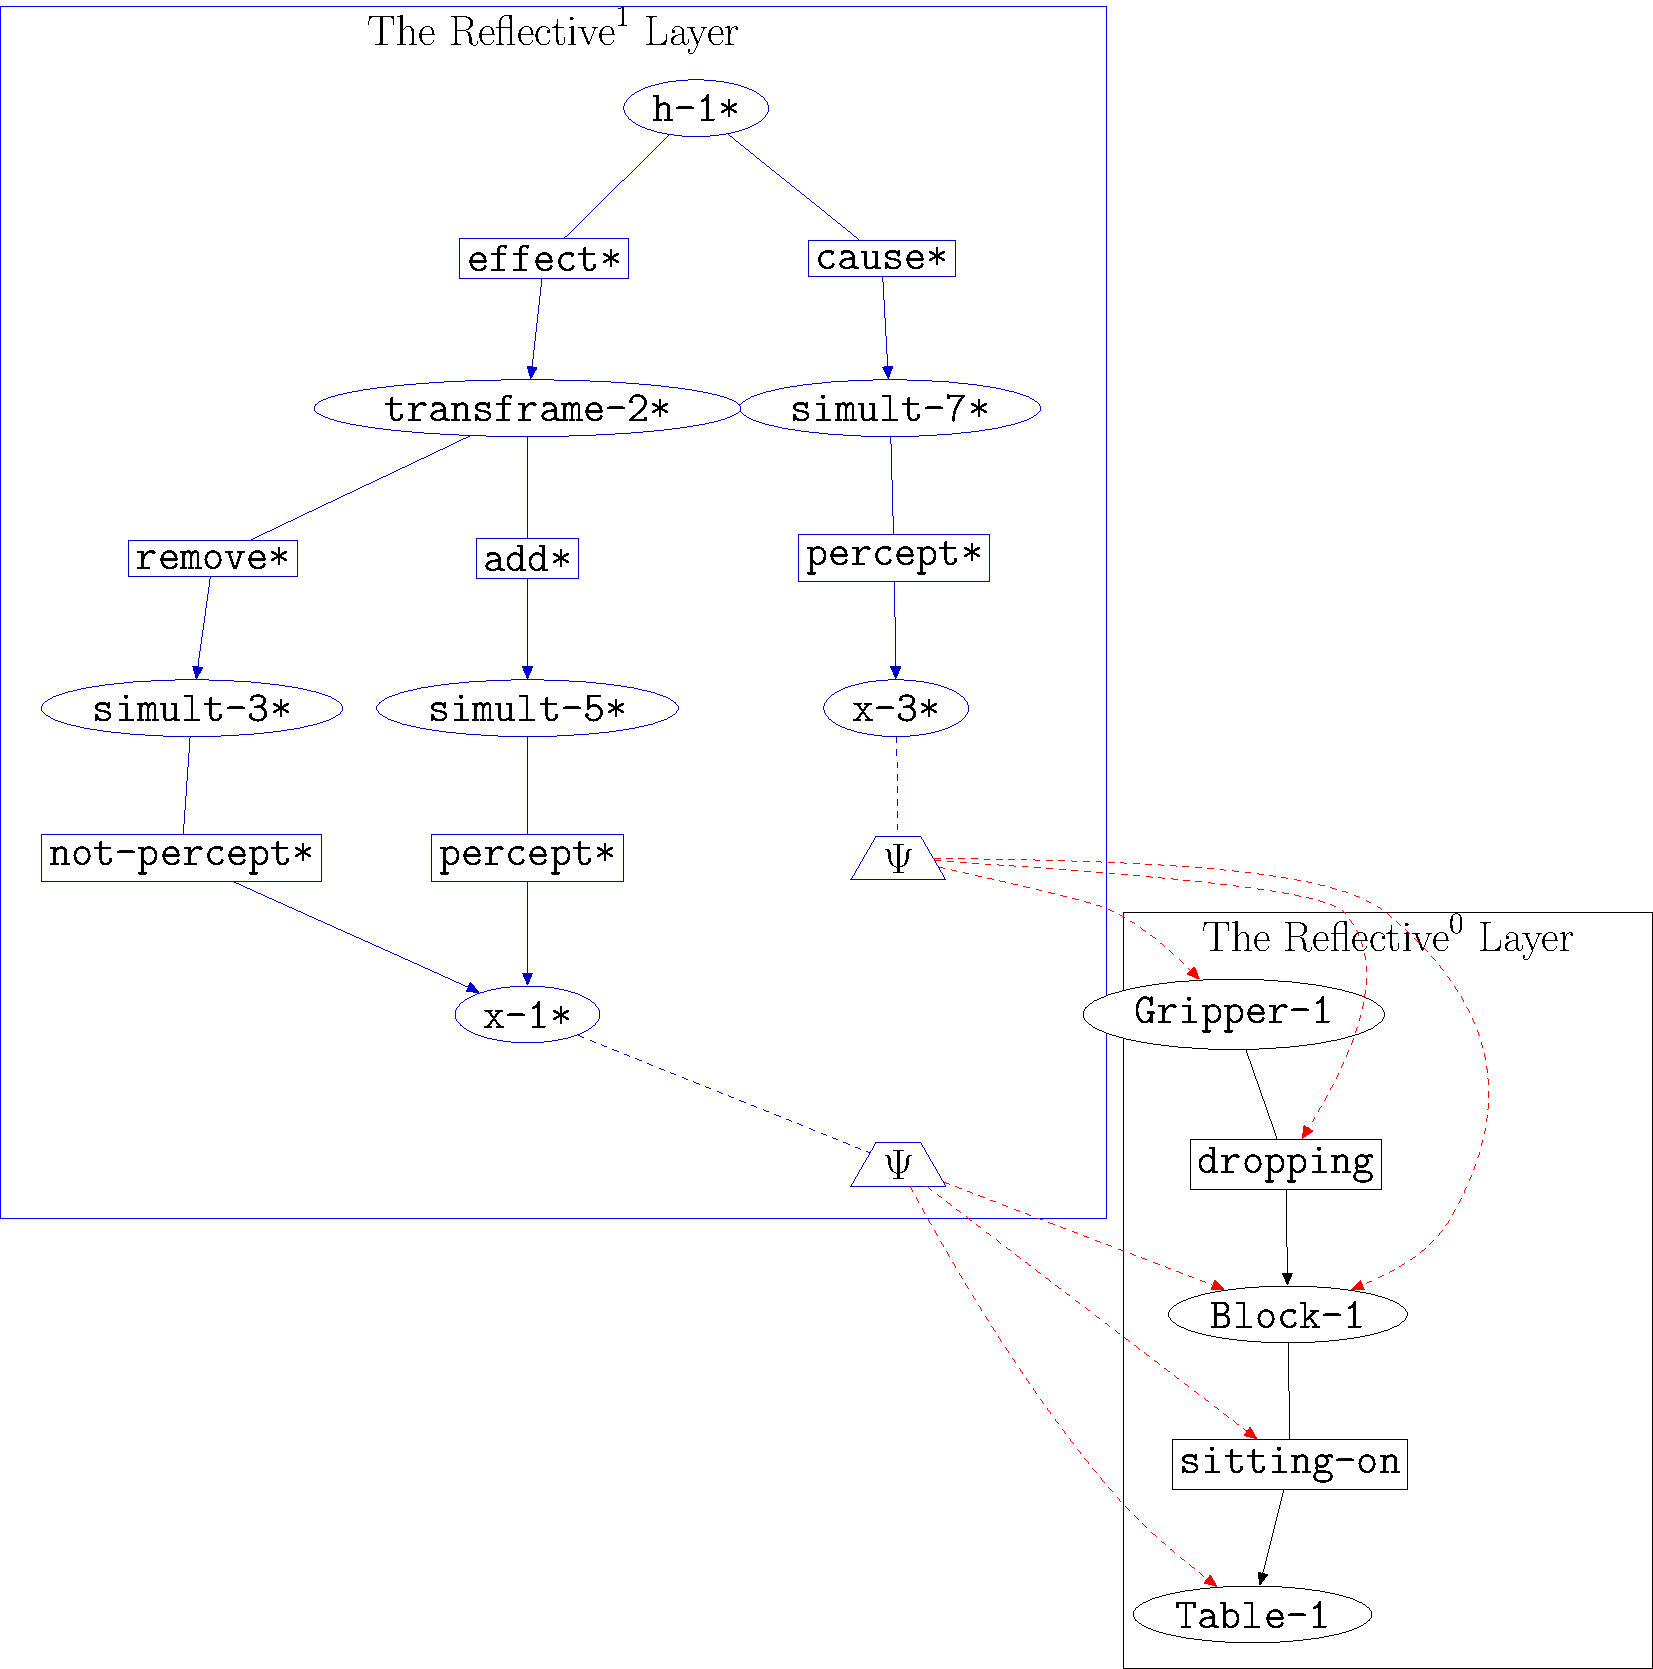
\includegraphics[width=8cm]{gfx/example_causal_hypothesis}
%\caption[An example of a causal hypothesis.]{An example of a causal
%  hypothesis, $h_1^*$, where the simultaneity,
%  $\text{\tt{simult}}_7^*$, is hypothesized to be the cause of the
%  transframe, $\text{\tt{transframe}}_2^*$.  In other words, the
%  gripper dropping the block causes the block to be sitting on the
%  table.}
%\label{figure:example_causal_hypothesis}
%\end{figure}


